% ************ Chapter 6 ************
%\renewcommand{\chaptername}{Chapter}

\chapter{Experimentação e Avaliação}
\label{cap:6}

\section{Experiências e Testes}
Neste contexto, uma experiência ou teste, assim como definido na secção \ref{estado_arte_avaliacao}, consiste na utilizando uma metodologia ou técnica específica de forma a avaliar uma determinada grandeza.

Assim, para a realização de um teste é preciso definir as grandezas, as hipóteses e as metodologias de avaliação.

\subsection{Grandezas a Avaliar}
Os objetivos definidos na secção \ref{objetivos} induzem uma contribuição para o projeto \emph{Solid} com vista a incrementar o seu potencial de escalabilidade, e desta forma cumprir, também, as hipóteses formuladas na secção \ref{section_hypothesis}.

Tendo isto em consideração, existem duas potenciais grandezas a avaliar:
\begin{itemize}
    \item Qualidade da implementação - A qualidade da implementação é crucial para tornar viável a aceitação da solução como uma contribuição para a comunidade em volta do Solid. A qualidade deverá ser mensurada tendo em conta métricas como resultados de software;
    \item Performance - Tendo em conta o mesmo escalamento, é relevante conseguir apurar se a solução desenvolvida consegue melhores resultados em termos de performance;
    \item Escalabilidade - Como complemento ponto referente à performance, é importante perceber se de facto a solução implementada é mais escalável horizontalmente que a plataforma atual.
\end{itemize}

\subsection{Hipóteses \label{avaliacao_experimentacao_hypothesis}}
Uma hipótese consiste numa afirmação que se quer corroborar através de testes estatísticos utilizando grandezas identificadas.

No contexto deste projeto, foram definidas duas hipóteses em linha com aquelas que foram formuladas na secção \ref{section_hypothesis}:
\begin{itemize}
    \item H1 - Hipótese referente a testes aplicacionais - Sucesso 100\% dos testes de software e cobertura superior a 80\%. Este valor vai em linha com o valor recomendado para criar um balanço entre cobertura de cenários de utilização e cobertura de código testado \cite{code_coverage};
    \item H2 - Hipótese referente a testes de performance - Capacidade de cada micro-serviço deve ser de pelo menos 75\% da suportada pela plataforma atual (monolítico) para uma determinada carga, mantendo o tempo máximo de resposta de cada pedido inferior a 400 milissegundos.
    O racional para a escolha do valor de 75\% surge no sentido de que podemos assumir que a performance individual dos serviços pode ser um pouco inferior do que o monólito, sem que isso afete o sistema orientado a micro-serviços como um todo, na medida em que o fator de escalabilidade flexível irá garantir melhor performance que o monólito.
    Por outro lado, o valor de 400 milissegundos foi obtido a partir da exploração das médias de tempo resposta para um conjunto basto de aplicações web através da fonte \cite{average_server_response_time}.
\end{itemize}

\subsection{Metodologias de Avaliação}
As metodologias de avaliação consistem na forma como serão verificadas as hipóteses definidas. A metodologia a utilizar irá depender da hipótese e da grandeza em causa.

A hipótese referente a testes aplicacionais, tendo em conta a qualidade da solução implementada, deve recorrer a testes de software, nomeadamente testes unitários e testes de integração que são executados através de ferramentas específicas para este efeito. Tendo em conta que esta metodologia é directa, não deverá ser necessário tratamento estatístico \cite{software_testing_2}.

A hipótese referente a testes de performance consiste em corroborar que cada micro-serviço do sistema, sob uma determinada carga, consegue suportar pelo menos 75\% do \emph{throughput} da plataforma atual (monólito), mantendo o tempo de resposta de cada pedido abaixo de 400 milissegundos.

Para esta hipótese deverão ser realizados testes de performance e capacidade aos diferentes micro-serviços e à plataforma atual.

Estes testes deverão ser executados recorrendo a ferramentas para este efeito (como por exemplo JMeter) e os resultados devem ser apontados de forma a poderem ser tiradas conclusões.

É importante referir que no caso dos micro-serviços, é expectável que os pedidos realizados durante os testes de carga passem pela \emph{API-Gateway}, de forma a que o cenário se aproxime o mais possível da realidade.

\section{Resultados}
Definidas as hipóteses e os meios e as metodologias de avaliação, seguem-se os resultados para cada uma das hipóteses propostas.

\subsection{Hipótese referente a testes aplicacionais}
Esta hipótese indica que os testes de Software devem ter uma taxa de sucesso de 100\%, bem como uma cobertura superior a 80\%.
No contexto da implementação foram utilizadas as bibliotecas \emph{mocha} e \emph{chai} para criar e mensurar os testes, tanto unitários como de integração.

Os números apresentados na tabela \ref{table_testes_aplicacionais_micro_services} correspondem ao conjunto de todos os projetos e bibliotecas externas alteradas no decorrer da implementação desta nova arquitetura para o Solid (\emph{c.f.} secção \ref{section_contribuicoes_investigacao}).
Numa perspetiva de estabelecer um ponto de comparação para perceber se existem diferenças substanciais nos números de testes e percentagem face à solução monolítica.

\begin{table}[h]
\centering
\caption{Resultados dos testes aplicacionais \emph{Solid} monólito}
\vspace{0.5cm}
\label{table_testes_aplicacionais_monolito}
\begin{tabular}{c|c|c|c} 
Testes Unitários & Testes de Integração & Cobertura \\
\hline                          
305 & 451 & 80\% \\
\end{tabular}
\end{table}

\begin{table}[h]
\centering
\caption{Resultados dos testes aplicacionais \emph{Solid} micro-seviços}
\vspace{0.5cm}
\label{table_testes_aplicacionais_micro_services}
\begin{tabular}{c|c|c|c} 
Testes Unitários & Testes de Integração & Cobertura \\
\hline                          
382 & 466 & 82\% \\
\end{tabular}
\end{table}

Com base nos resultados apresentados na tabela \ref{table_testes_aplicacionais_micro_services} é possível inferir que tanto a taxa de sucesso como a taxa de cobertura permitem corroborar a hipótese estipulada.

Na mesma linha de raciocínio, quando comparados estes valores com os correspondentes à solução monolítica (\emph{c.f.} tabela \ref{table_testes_aplicacionais_monolito}) é possível perceber que houve uma ligeira melhoria tanto em termos de cobertura como em número de testes realizados à plataforma.

\subsection{Hipótese referente a testes de performance}
A segunda hipótese incide na análise de performance dos micro-serviços desenvolvidos, com vista a inferir se houve de facto ganhos justificativos em relação à arquitetura atual.

\subsubsection*{\emph{Setup} dos Testes \label{section_setup_testes}}

A premissa base foi de que tanto o monólito, como os micro-serviços seriam testados estando a ser executados apenas numa instância sem qualquer tipo de escalamento, isto porque o monólito não suporta escalamento horizontal e, desta forma os resultados obtidos poderiam não ser fiáveis. 

Esta premissa vai de encontro à hipótese referente a performance do sistema desenvolvido, formulada na secção \ref{section_hypothesis}.

Para a realização dos testes foi utilizada a ferramenta de testes de carga \emph{JMeter}, que permite simular utilizadores e pedidos simultâneos a um determinado serviço. Esta ferramenta disponibiliza a funcionalidade de executar contra interfaces de aplicação \emph{\acrshort{REST}} através da configuração dos seguintes parâmetros:
\begin{itemize}
    \item Caminho - O caminho que permite chegar ao serviço;
    \item Método - Método HTTP do \emph{endpoint} específico;
    \item Numero de \emph{Threads} - Cada \emph{thread} permite simular um utilizador a executar pedidos, sendo que múltiplas \emph{threads} irão ser executadas em paralelo e, por consequência, simular múltiplos utilizadores a fazer pedidos em simultâneo;
    \item Período \emph{Ramp-up} - Variável em segundos que indica quão gradual devem ser criadas novas \emph{threads}. A divisão do numero de \emph{threads} pelo valor configurado nesta variável indica o numero de novas \emph{threads} que serão criadas por segundo até que seja atingido o numero total;
    \item Total repetições - Numero de pedidos que cada \emph{thread} irá fazer. Assim que todas terminarem de executar o valor total de repetições, está concluído.
\end{itemize}

De forma a perceber o numero de utilizadores simultâneos que deveriam ser configurados, foram efectuados sucessivos testes de performance com incremento do número de \emph{threads} e, assim, perceber qual o número máximo de utilizadores simultâneos que uma instância de \emph{Solid} consegue servir mantendo um tempo de resposta inferior a 400milissegundos.

\begin{table}[h]
\centering
\caption{Tabela configurações base JMeter}
\vspace{0.5cm}
\label{jmeter_configs}
\begin{tabular}{c|c|c|c} 
 Número de \emph{threads} & Período \emph{Ramp-up} & Número Repetições \\
\hline                          
10 & 10 & 200 \\
\end{tabular}
\end{table}

Utilizando as configurações da tabela \ref{jmeter_configs}, ao fim de 10 segundos teremos 10 utilizadores simultâneos que irão fazer um total de 200 pedidos cada um.

De forma a manter a equidade em termos de \emph{hardware}, os diferentes serviços serão testados a executar em \emph{\acrfull{VPS}} adquiridos apenas para estas experiências, com as configurações base referidas na tabela \ref{vps_configs}.

\begin{table}[h]
\centering
\caption{Tabela configurações base \emph{\acrshort{VPS}}}
\vspace{0.5cm}
\label{vps_configs}
\begin{tabular}{c|c|c|c|} 
CPU & RAM & Disco & Sistema Operativo \\
\hline                          
2 cores & 4GB & 50GB SSD & CentOS 7 \\
\end{tabular}
\end{table}

Estas experiências deverão incidir, por um lado, sobre casos de uso que permitam exercitar os diferentes micro-serviços na arquitetura proposta ({c.f.} secção \ref{section_arquitetura_proposta}), e, por outro lado, sobre casos de uso que representem funcionalidades cruciais para o \emph{\acrshort{POD}}. Assim, os testes de performance irão incidir sobre três casos de uso:
\begin{itemize}
    \item Criação de uma nova conta
    \item Autenticação
    \item Obter recurso
\end{itemize}

No caso do monólito, o teste deverá incidir sobre a mesma instância aplicacional para os \emph{endpoints} correspondentes aos três pedidos de forma simultânea, permitindo simular circunstâncias o mais reais possíveis.

Para a arquitetura orientada a micro-serviços, estes testes deverão fazer incidir os pedidos, de forma independente, nos serviços responsáveis pelos respetivos casos de uso:
\begin{itemize}
    \item \emph{Accounts Web} - Criação de uma nova conta;
    \item \emph{Solid ID Web} - Autenticação;
    \item \emph{Solid Storage Web} - Obter recurso.
\end{itemize}

\subsubsection*{Teste Monólito \label{section_tests_monolith}}

Para o teste de performance ao monólito foi implantado o sistema \emph{Solid} sob a arquitetura monolítica numa das \emph{\acrshort{VPS}} (\emph{c.f.} figura \ref{monolith_tests_implantation_diagram}). Estes testes incluíram, assim como proposto na secção \ref{section_setup_testes}, pedidos a três diferentes \emph{endpoints}, correspondentes a interações de registo de conta, autenticação e obtenção de recurso.

\begin{figure}[H]
    \begin{center}
    % Requires \usepackage{graphicx}
    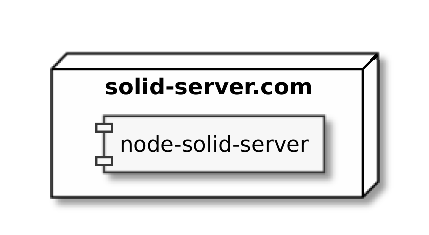
\includegraphics[width=0.3 \textwidth]{figures/monolith_tests.eps}
    \caption{Implantação \emph{solid server} monólito}
    \label{monolith_tests_implantation_diagram}
    \end{center}
\end{figure}

Os dados relevantes para este cenário de teste são o tempo médio de resposta (em milissegundos) e o \emph{throughput} (em pedidos/segundo), na medida em que estes são os dados que permitirão corroborar a hipótese formulada (\emph{c.f. tabela \ref{table_resultados_testes_performance_monolith}}).

\begin{table}[h]
\centering

\caption{Resultados teste performance \emph{solid server} monólito}
\label{table_resultados_testes_performance_monolith}
\vspace{0.5cm}
\begin{tabular}{c|c|c|c}
 - & Média tempo de resposta (ms) & \emph{Throughput} (p/s) \\
\hline                          
Total & 380 & 20.6 \\
\end{tabular}
\end{table}

\subsubsection*{Teste arquitetura micro-serviços em apenas um nó \label{tests_micro_services_1}}

Para este cenário de teste a solução orientada a micro-serviços (\emph{c.f.} secção  \ref{section_arquitetura_proposta}) seguiu uma implantação em apenas um nó, como é possível observar na figura \ref{figure_micro_services_tests_1_implantation_diagram}.

\begin{figure}[H]
    \begin{center}
    \label{figure_micro_services_tests_1_implantation_diagram}
    % Requires \usepackage{graphicx}
    
\includegraphics[width=1 \textwidth]{figures/microservices_tests1.eps}
    \caption{Implantação arquitetura orientada a micro-serviços em apenas um nó}
    \end{center}
\end{figure}


Os resultados para este teste são apresentados na tabela \ref{r_t_m_s_1}, incluindo para cada um dos micro-serviços, os valores de tempo médio de resposta e \emph{throughput}.
Conforme é possível perceber, face aos resultados do teste ao monólito expostos na tabela \ref{monolith_tests_implantation_diagram}, os valores demonstram perdas significativas em ambas as métricas, colocando, assim, em risco a inferência da hipótese formulada no âmbito dos testes de performance (\emph{c.f.} \ref{avaliacao_experimentacao_hypothesis}).

\begin{table}[h]
\centering
\caption{Resultados teste de performance a arquitetura micro-serviços instalada em apenas um nó}
\label{r_t_m_s_1}
\vspace{0.5cm}
\begin{tabular}{c|c|c|c} 
 - & Tempo médio de resposta (ms) & \emph{Throughput} (p/s) \\
\hline                          
\emph{Solid ID Web} & 524 & 11.2 \\
\emph{Solid Storage Web} & 600 & 12 \\
 \emph{Accounts Web} & 490 & 14.2 \\
\end{tabular}
\end{table}

O facto de todos os micro-serviços, bem como o \emph{Message Broker} e o componente com a função de \emph{API Gateway}, terem sido instalados no mesmo nó (\emph{c.f} figura \ref{figure_micro_services_tests_1_implantation_diagram}), pode estar a criar alguma sobrecarga no nó e, consequentemente, resultar em perda de performance. Esta teoria, deve, por sua vez, ser também corroborada com base nos testes subsequentes.

\subsubsection*{Teste arquitetura micro-serviços distribuídos \label{tests_micro_services_2}}

Tendo em conta o resultados dos testes documentados na secção \ref{tests_micro_services_1} apresentarem perdas de performance significativas face aos valores obtidos para o monólito (\emph{c.f.} tabela \ref{table_resultados_testes_performance_monolith}), segue-se um novo teste com uma abordagem de implantação diferente.
Neste teste, o sistema \emph{Solid} sob arquitetura orientada a micro-serviços foi instalado seguindo uma implantação distribuída em mais do que um nó (\emph{c.f.} figura \ref{figure_solid_micro_services_multiples_vps_implantation_diagram}).

\begin{figure}[H]
    \begin{center}
    % Requires \usepackage{graphicx}
    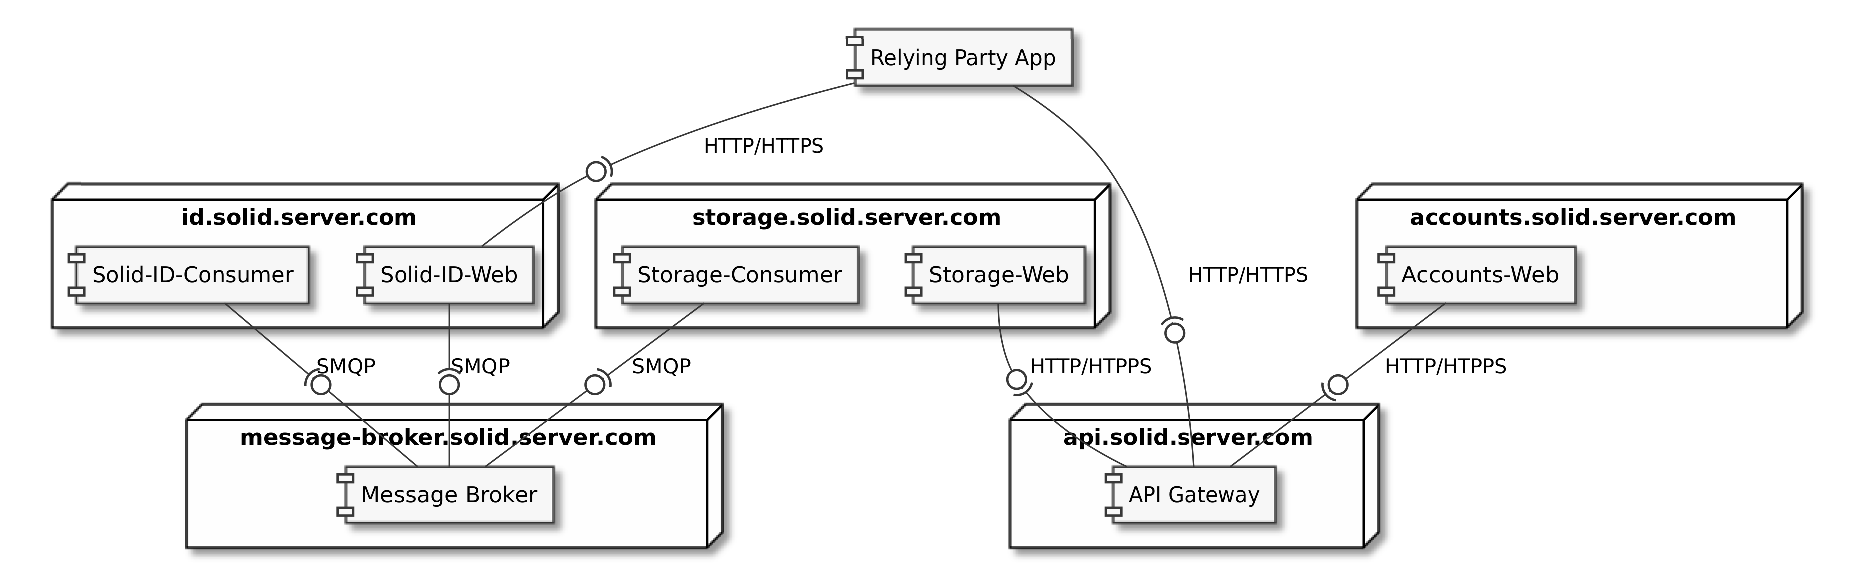
\includegraphics[width=1 \textwidth]{figures/microservices_tests2.eps}
    \caption{Implantação arquitetura orientada a micro-serviços distribuída}
    \label{figure_solid_micro_services_multiples_vps_implantation_diagram}
    \end{center}
\end{figure}


Os resultados para este cenário são apresentados sob a forma tabular para cada um dos micro-serviços em causa, seguindo assim o plano de \emph{setup} dos testes (\emph{c.f.} secção \ref{section_setup_testes}).

\begin{table}[h]
\centering
\caption{Resultados teste de performance a arquitetura micro-serviços distribuídos}
\label{r_t_m_s_2}
\vspace{0.5cm}
\begin{tabular}{c|c|c|c} 
 - & Média tempo de resposta (ms) & \emph{Throughput} (p/s) \\
\hline                          
\emph{Solid ID Web} & 390 & 16.2 \\
\emph{Solid Storage Web} & 385 & 17.6 \\
\emph{Accounts Web} & 320 & 19.6 \\
\end{tabular}
\end{table}

Com base nos valores apresentados na tabela \ref{r_t_m_s_2} é possível corroborar a teoria de que o \emph{hardware} terá sido o \emph{bottleneck nos testes} apresentados na secção \ref{tests_micro_services_1}, estando assim mitigado esse problema. É possível também perceber que os resultados dos testes para este cenário, apesar de apresentarem perdas menos significativas tanto a nível de tempo médio de resposta como de \emph{throughput}, revelam que podem, ainda, existir possíveis alterações à implantação com potencial de melhoria de performance.

\subsubsection*{Teste arquitetura micro-serviços distribuídos sem \emph{containers} \label{tests_micro_services_3}}

Conforme explicado, apesar dos resultados dos testes documentados na secção \ref{tests_micro_services_2} serem relativamente satisfatórios tendo em conta àquilo que foi estipulado pela hipótese formulada, segue-se um novo teste com uma abordagem de implantação sem recurso à tecnologia \emph{containers}.

Neste teste, o sistema \emph{Solid} sob arquitetura orientada a micro-serviços seguiu, tal como no teste \ref{tests_micro_services_2}, uma implantação distribuída em mais do que um nó (\emph{c.f.} figura \ref{figure_solid_micro_services_multiples_vps_implantation_diagram}), mas neste cenário não foi utilizada qualquer tecnologia de \emph{containers}, estando os serviços a ser executados diretamente sobre o sistema operativo da máquina.

\begin{table}[h]
\centering
\caption{Resultados teste performance a arquitetura micro-serviços distribuídos sem \emph{containers}}
\label{r_t_m_s_3}
\vspace{0.5cm}
\begin{tabular}{c|c|c|c} 
 - & Média tempo de resposta (ms) & \emph{Throughput} (p/s) \\
\hline                          
\emph{Solid ID Web} & 385 & 19.0 \\
\emph{Solid Storage Web} & 370 & 20.2 \\
\emph{Accounts Web} & 300 & 22.6 \\
\end{tabular}
\end{table}

Os resultados apresentados na tabela \ref{r_t_m_s_3} parecem corroborar a teoria de que a tecnologia \emph{containers}, apesar das vantagens referidas na secção \ref{estado_arte_containers}, cria alguma latência que terá tido algum impacto nos testes da secção \ref{tests_micro_services_2}. No mesmo contexto, estes valores estão, já, bastante próximos aos valores resultantes dos testes relativos ao \emph{Solid} monolítico, apresentando até, em grande parte dos casos, algumas melhorias.

\section{Sumário}
Com base nos testes de performance realizados ao monólito (\emph{c.f.} tabela \ref{table_resultados_testes_performance_monolith}), foi possível obter um \emph{throughput} de 20.6 pedidos por segundo com uma média de tempo de resposta de 380ms, desta forma, segundo a hipótese formulada, o valor de \emph{throughput} para os micro-serviços deverá ser no mínimo de 75\% esse valor, ou seja, superior a 15.45 pedidos por segundo e mantendo um tempo médio de resposta inferior a 400ms.

A tabela \ref{tabela_resultados_aglomerados} foi construída com o objetivo de, tendo por base testes realizados ao \emph{Solid} monolítico (\emph{c.f.} secção \ref{section_tests_monolith}), salientar as evoluções percentuais dos valores de tempo médio de resposta e \emph{Throughput} para os diferentes testes realizados à arquitetura orientada a micro-serviços:
\begin{itemize}
    \item este arquitetura micro-serviços em apenas um nó (\emph{c.f.} secção \ref{tests_micro_services_1});
    \item Teste arquitetura micro-serviços distribuídos (\emph{c.f.}\ref{tests_micro_services_2});
    \item Teste arquitetura micro-serviços distribuídos sem \emph{containers} (\emph{c.f.} secção \ref{tests_micro_services_3}).
\end{itemize}

\begin{center}
\begin{table}[h]
\caption{Tabela de resultados percentuais dos testes face ao teste realizado ao \emph{Solid} monolítico}
\label{tabela_resultados_aglomerados}
 \centering
 \begin{tabular}{|c|l|c|c|c|c|}
 \hline
 & \multicolumn{1}{c|}{} & \multicolumn{1}{c|}{\specialcell{Evolução\\Tempo médio\\de resposta\\(\%)}} & \multicolumn{1}{c|}{\specialcell{Evolução\\\emph{Throughput}\\(\%)}}\\
 \hline
\multirow{3}{*}{\specialcell{Micro-serviços\\apenas um nó}} & \emph{Solid ID Web} &-39&-46\\
 & \emph{Solid Storage Web} &-58&-42\\
 & \emph{Accounts Web} &-29&-31\\
 \hline
 \multirow{3}{*}{\specialcell{Micro-serviços\\distribuídos}} & \emph{Solid ID Web} &-3&-21\\
 & \emph{Solid Storage Web} &-1&-15\\
 & \emph{Accounts Web} &16&-5\\
 \hline
 \multirow{3}{*}{\specialcell{Micro-serviços\\distribuídos sem\\\emph{containers}}} & \emph{Solid ID Web} &1&-8\\
 & \emph{Solid Storage Web} &-1&-2\\
 & \emph{Accounts Web} &21&10\\
 \hline
 \end{tabular}
 \end{table}
\end{center}

O primeiro teste aos micro-serviços seguiu uma implantação relativamente simples e com potencial de custos reduzidos, tendo sido toda a arquitetura implantada numa única máquina.

Porém, utilizando esta solução sem qualquer tipo de escalamento vertical ou horizontal, acaba por tornar o \emph{hardware} o \emph{bottleneck} da arquitetura, afetando tanto o \emph{throughput} como o tempo médio de resposta de cada pedido processado.

Tendo em conta que o teste anterior não cumpre com as metas inferidas nesta hipótese, um novo teste foi desenhado recorrendo a uma implantação distribuída (\emph{c.f.} figura \ref{figure_solid_micro_services_multiples_vps_implantation_diagram}), mantendo, desta forma, a premissa de não recorrer nestes testes a escalamento vertical ou horizontal e ao mesmo tempo eliminar o \emph{bottleneck} do \emph{hardware}.

Os resultados deste segundo teste foram mais satisfatórios e permitem inferior que esta hipótese está também cumprida. Os resultados um pouco inferiores aos do monólito podem ser explicados pelo facto dos micro-serviços estarem a ser executados sobre um ambiente de \emph{containers} com a tecnologia \emph{docker}, sendo esta ultima teoria comprovada com base nos testes apresentados na secção \ref{tests_micro_services_3}.

Estes resultados permitem, desta forma, aferir que o sistema desenvolvido confere, garantindo a mesma experiência de utilização, uma performance não inferior quando submetido às mesmas condições de escalamento horizontal e vertical, corroborando os pressupostos adjacentes a esta dissertação (\emph{c.f. secção \ref{section_hypothesis}}).






